\documentclass[twoside]{book}

% Packages required by doxygen
\usepackage{fixltx2e}
\usepackage{calc}
\usepackage{doxygen}
\usepackage{graphicx}
\usepackage[utf8]{inputenc}
\usepackage{makeidx}
\usepackage{multicol}
\usepackage{multirow}
\PassOptionsToPackage{warn}{textcomp}
\usepackage{textcomp}
\usepackage[nointegrals]{wasysym}
\usepackage[table]{xcolor}

% Font selection
\usepackage[T1]{fontenc}
\usepackage{mathptmx}
\usepackage[scaled=.90]{helvet}
\usepackage{courier}
\usepackage{amssymb}
\usepackage{sectsty}
\renewcommand{\familydefault}{\sfdefault}
\allsectionsfont{%
  \fontseries{bc}\selectfont%
  \color{darkgray}%
}
\renewcommand{\DoxyLabelFont}{%
  \fontseries{bc}\selectfont%
  \color{darkgray}%
}
\newcommand{\+}{\discretionary{\mbox{\scriptsize$\hookleftarrow$}}{}{}}

% Page & text layout
\usepackage{geometry}
\geometry{%
  a4paper,%
  top=2.5cm,%
  bottom=2.5cm,%
  left=2.5cm,%
  right=2.5cm%
}
\tolerance=750
\hfuzz=15pt
\hbadness=750
\setlength{\emergencystretch}{15pt}
\setlength{\parindent}{0cm}
\setlength{\parskip}{0.2cm}
\makeatletter
\renewcommand{\paragraph}{%
  \@startsection{paragraph}{4}{0ex}{-1.0ex}{1.0ex}{%
    \normalfont\normalsize\bfseries\SS@parafont%
  }%
}
\renewcommand{\subparagraph}{%
  \@startsection{subparagraph}{5}{0ex}{-1.0ex}{1.0ex}{%
    \normalfont\normalsize\bfseries\SS@subparafont%
  }%
}
\makeatother

% Headers & footers
\usepackage{fancyhdr}
\pagestyle{fancyplain}
\fancyhead[LE]{\fancyplain{}{\bfseries\thepage}}
\fancyhead[CE]{\fancyplain{}{}}
\fancyhead[RE]{\fancyplain{}{\bfseries\leftmark}}
\fancyhead[LO]{\fancyplain{}{\bfseries\rightmark}}
\fancyhead[CO]{\fancyplain{}{}}
\fancyhead[RO]{\fancyplain{}{\bfseries\thepage}}
\fancyfoot[LE]{\fancyplain{}{}}
\fancyfoot[CE]{\fancyplain{}{}}
\fancyfoot[RE]{\fancyplain{}{\bfseries\scriptsize Generated on Thu Sep 8 2016 13\+:04\+:28 for Passive D\+S Control by Doxygen }}
\fancyfoot[LO]{\fancyplain{}{\bfseries\scriptsize Generated on Thu Sep 8 2016 13\+:04\+:28 for Passive D\+S Control by Doxygen }}
\fancyfoot[CO]{\fancyplain{}{}}
\fancyfoot[RO]{\fancyplain{}{}}
\renewcommand{\footrulewidth}{0.4pt}
\renewcommand{\chaptermark}[1]{%
  \markboth{#1}{}%
}
\renewcommand{\sectionmark}[1]{%
  \markright{\thesection\ #1}%
}

% Indices & bibliography
\usepackage{natbib}
\usepackage[titles]{tocloft}
\setcounter{tocdepth}{3}
\setcounter{secnumdepth}{5}
\makeindex

% Hyperlinks (required, but should be loaded last)
\usepackage{ifpdf}
\ifpdf
  \usepackage[pdftex,pagebackref=true]{hyperref}
\else
  \usepackage[ps2pdf,pagebackref=true]{hyperref}
\fi
\hypersetup{%
  colorlinks=true,%
  linkcolor=blue,%
  citecolor=blue,%
  unicode%
}

% Custom commands
\newcommand{\clearemptydoublepage}{%
  \newpage{\pagestyle{empty}\cleardoublepage}%
}


%===== C O N T E N T S =====

\begin{document}

% Titlepage & ToC
\hypersetup{pageanchor=false,
             bookmarks=true,
             bookmarksnumbered=true,
             pdfencoding=unicode
            }
\pagenumbering{roman}
\begin{titlepage}
\vspace*{7cm}
\begin{center}%
{\Large Passive D\+S Control }\\
\vspace*{1cm}
{\large Generated by Doxygen 1.8.7}\\
\vspace*{0.5cm}
{\small Thu Sep 8 2016 13:04:28}\\
\end{center}
\end{titlepage}
\clearemptydoublepage
\tableofcontents
\clearemptydoublepage
\pagenumbering{arabic}
\hypersetup{pageanchor=true}

%--- Begin generated contents ---
\chapter{My Personal Index Page}
\label{index}\hypertarget{index}{}Implementation of various controllers for using D\+S task models on real robots. Refer to the publication K. Kronander and A. Billard; Passive Interaction Control with Dynamical Systems; I\+E\+E\+E Robotics and Automation Letters 2016 
\chapter{R\+E\+A\+D\+M\+E}
\label{md_README}
\hypertarget{md_README}{}
passive D\+S control

\href{https://magnum.travis-ci.com/epfl-lasa/passive-ds-control}{\tt !\mbox{[}Build Status\mbox{]}(https\+://magnum.\+travis-\/ci.\+com/epfl-\/lasa/passive-\/ds-\/control.\+svg?token=\+Bq\+U\+Qb763ts\+V\+V4\+Qyz\+Lg\+By\&branch=master)}

Package for robot toolkit. 
\chapter{Hierarchical Index}
\section{Class Hierarchy}
This inheritance list is sorted roughly, but not completely, alphabetically\+:\begin{DoxyCompactList}
\item \contentsline{section}{Cascade\+D\+S\+Controller}{\pageref{classCascadeDSController}}{}
\item \contentsline{section}{D\+S\+Controller}{\pageref{classDSController}}{}
\begin{DoxyCompactList}
\item \contentsline{section}{Passive\+D\+S\+Controller}{\pageref{classPassiveDSController}}{}
\end{DoxyCompactList}
\item \contentsline{section}{Openloop\+D\+S\+Controller}{\pageref{classOpenloopDSController}}{}
\item \contentsline{section}{Smooth\+Rise2d}{\pageref{classSmoothRise2d}}{}
\item \contentsline{section}{Smooth\+Rise\+Fall}{\pageref{classSmoothRiseFall}}{}
\item \contentsline{section}{Smooth\+Rise\+Fall2d}{\pageref{classSmoothRiseFall2d}}{}
\end{DoxyCompactList}

\chapter{Class Index}
\section{Class List}
Here are the classes, structs, unions and interfaces with brief descriptions\+:\begin{DoxyCompactList}
\item\contentsline{section}{\hyperlink{classCascadeDSController}{Cascade\+D\+S\+Controller} }{\pageref{classCascadeDSController}}{}
\item\contentsline{section}{\hyperlink{classDSController}{D\+S\+Controller} }{\pageref{classDSController}}{}
\item\contentsline{section}{\hyperlink{classOpenloopDSController}{Openloop\+D\+S\+Controller} }{\pageref{classOpenloopDSController}}{}
\item\contentsline{section}{\hyperlink{classPassiveDSController}{Passive\+D\+S\+Controller} }{\pageref{classPassiveDSController}}{}
\item\contentsline{section}{\hyperlink{classSmoothRise2d}{Smooth\+Rise2d} }{\pageref{classSmoothRise2d}}{}
\item\contentsline{section}{\hyperlink{classSmoothRiseFall}{Smooth\+Rise\+Fall} }{\pageref{classSmoothRiseFall}}{}
\item\contentsline{section}{\hyperlink{classSmoothRiseFall2d}{Smooth\+Rise\+Fall2d} }{\pageref{classSmoothRiseFall2d}}{}
\end{DoxyCompactList}

\chapter{Class Documentation}
\hypertarget{classCascadeDSController}{\section{Cascade\+D\+S\+Controller Class Reference}
\label{classCascadeDSController}\index{Cascade\+D\+S\+Controller@{Cascade\+D\+S\+Controller}}
}
\subsection*{Public Member Functions}
\begin{DoxyCompactItemize}
\item 
\hypertarget{classCascadeDSController_a291701f57a7fc001d2dbc0edef0c65f2}{{\bfseries Cascade\+D\+S\+Controller} (size\+\_\+t dim, std\+::function$<$ Vec(Vec)$>$ task\+\_\+dynamics, std\+::function$<$ Vec(Vec)$>$ process\+\_\+filter)}\label{classCascadeDSController_a291701f57a7fc001d2dbc0edef0c65f2}

\item 
\hypertarget{classCascadeDSController_a69aef025bd5c8bbea34958b649fb0452}{void {\bfseries Forward\+Integration} (realtype driving\+\_\+force, const Mat \&stiffness, realtype dt, realtype speed\+\_\+threshold)}\label{classCascadeDSController_a69aef025bd5c8bbea34958b649fb0452}

\item 
\hypertarget{classCascadeDSController_a1e51fe3a3652228c4cfb50cbcce98451}{void {\bfseries Reset} (const Vec \&act\+\_\+pos, int n\+\_\+burn=N\+\_\+\+B\+U\+R\+N)}\label{classCascadeDSController_a1e51fe3a3652228c4cfb50cbcce98451}

\item 
\hypertarget{classCascadeDSController_a69cb5e84d7f34c628627819dce8ead36}{Mat {\bfseries Integrate\+Trajectory} (realtype dt, realtype speed\+\_\+threshold, realtype t\+\_\+max)}\label{classCascadeDSController_a69cb5e84d7f34c628627819dce8ead36}

\item 
\hypertarget{classCascadeDSController_ae19aca7dfdac51d61bdf61d71c41af71}{void {\bfseries Update} (const Vec \&act\+\_\+pos)}\label{classCascadeDSController_ae19aca7dfdac51d61bdf61d71c41af71}

\item 
\hypertarget{classCascadeDSController_a7d099821e73094bf63fa3d8bd776cdcf}{Vec {\bfseries ref\+\_\+pos} ()}\label{classCascadeDSController_a7d099821e73094bf63fa3d8bd776cdcf}

\item 
\hypertarget{classCascadeDSController_ac179e9eccd277656fc7dcd6ffb7baf78}{size\+\_\+t {\bfseries dim} ()}\label{classCascadeDSController_ac179e9eccd277656fc7dcd6ffb7baf78}

\item 
\hypertarget{classCascadeDSController_a090f174c8f1f7f91733cf694e3f96833}{void {\bfseries set\+\_\+ds\+\_\+origin} (const Vec \&ds\+\_\+origin)}\label{classCascadeDSController_a090f174c8f1f7f91733cf694e3f96833}

\end{DoxyCompactItemize}


The documentation for this class was generated from the following files\+:\begin{DoxyCompactItemize}
\item 
include/cascade\+\_\+ds\+\_\+controller.\+h\item 
src/cascade\+\_\+ds\+\_\+controller.\+cpp\end{DoxyCompactItemize}

\hypertarget{classDSController}{\section{D\+S\+Controller Class Reference}
\label{classDSController}\index{D\+S\+Controller@{D\+S\+Controller}}
}


Inheritance diagram for D\+S\+Controller\+:\nopagebreak
\begin{figure}[H]
\begin{center}
\leavevmode
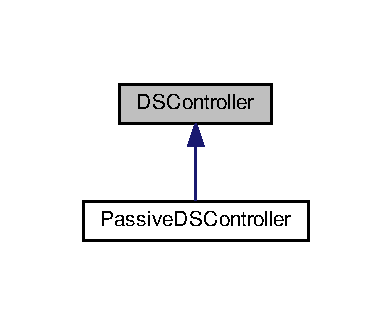
\includegraphics[width=188pt]{classDSController__inherit__graph}
\end{center}
\end{figure}
\subsection*{Public Member Functions}
\begin{DoxyCompactItemize}
\item 
\hypertarget{classDSController_a58f137f5163f7e5446ed3bbb6f51dd84}{{\bfseries D\+S\+Controller} (int dim, realtype damping\+\_\+eigval0, realtype damping\+\_\+eigval1)}\label{classDSController_a58f137f5163f7e5446ed3bbb6f51dd84}

\item 
\hypertarget{classDSController_a16d6380a8cd8be3b50742770c5d1b469}{Mat {\bfseries Compute\+Damping} (const Vec \&ref\+\_\+vel)}\label{classDSController_a16d6380a8cd8be3b50742770c5d1b469}

\item 
\hypertarget{classDSController_ad378ee521f62f3832781bf9341dadb3e}{void {\bfseries Compute\+Orthonormal\+Basis} (const Vec \&dir)}\label{classDSController_ad378ee521f62f3832781bf9341dadb3e}

\item 
\hypertarget{classDSController_a8a7fc8de1b4fa9aa5e53d00f02c1a8ef}{void {\bfseries Update} (const Vec \&vel, const Vec \&ref\+\_\+vel)}\label{classDSController_a8a7fc8de1b4fa9aa5e53d00f02c1a8ef}

\item 
\hypertarget{classDSController_ab08bcc5c458aa127c1527f21f4525de8}{void {\bfseries set\+\_\+damping\+\_\+eigval} (realtype damping\+\_\+eigval0, realtype damping\+\_\+eigval1)}\label{classDSController_ab08bcc5c458aa127c1527f21f4525de8}

\item 
\hypertarget{classDSController_a33a08c811cc77253674951282221ee92}{void {\bfseries set\+\_\+damping\+\_\+eigval} (const Mat \&damping\+\_\+eigval)}\label{classDSController_a33a08c811cc77253674951282221ee92}

\item 
\hypertarget{classDSController_aa0ac90880dc0e6a379da8545fe909bc1}{Mat {\bfseries damping\+\_\+eigval} () const }\label{classDSController_aa0ac90880dc0e6a379da8545fe909bc1}

\item 
\hypertarget{classDSController_ab9be9f5e11c3b57b3263334fe2ee91a0}{Vec {\bfseries control\+\_\+output} () const }\label{classDSController_ab9be9f5e11c3b57b3263334fe2ee91a0}

\end{DoxyCompactItemize}
\subsection*{Protected Attributes}
\begin{DoxyCompactItemize}
\item 
\hypertarget{classDSController_aad5c60f1f2bb0778ac3a801e730e1722}{Mat {\bfseries damping\+\_\+}}\label{classDSController_aad5c60f1f2bb0778ac3a801e730e1722}

\item 
\hypertarget{classDSController_a6f862346b14a9341c5702f5d63f08d93}{Mat {\bfseries basis\+\_\+}}\label{classDSController_a6f862346b14a9341c5702f5d63f08d93}

\item 
\hypertarget{classDSController_aad418cf55e7f8f6f65b475bbd56550b6}{Mat {\bfseries damping\+\_\+eigval\+\_\+}}\label{classDSController_aad418cf55e7f8f6f65b475bbd56550b6}

\item 
\hypertarget{classDSController_a04a9628bdf15d1891bf883b1c1e456b5}{Vec {\bfseries control\+\_\+output\+\_\+}}\label{classDSController_a04a9628bdf15d1891bf883b1c1e456b5}

\end{DoxyCompactItemize}


The documentation for this class was generated from the following files\+:\begin{DoxyCompactItemize}
\item 
include/passive\+\_\+ds\+\_\+controller.\+h\item 
src/passive\+\_\+ds\+\_\+controller.\+cpp\end{DoxyCompactItemize}

\hypertarget{classOpenloopDSController}{\section{Openloop\+D\+S\+Controller Class Reference}
\label{classOpenloopDSController}\index{Openloop\+D\+S\+Controller@{Openloop\+D\+S\+Controller}}
}
\subsection*{Public Member Functions}
\begin{DoxyCompactItemize}
\item 
\hypertarget{classOpenloopDSController_a7c98b3506a67b133cdc148e974a2ff56}{{\bfseries Openloop\+D\+S\+Controller} (size\+\_\+t dim, std\+::function$<$ Vec(Vec)$>$ task\+\_\+dynamics)}\label{classOpenloopDSController_a7c98b3506a67b133cdc148e974a2ff56}

\item 
\hypertarget{classOpenloopDSController_a50e5440134b967ba4937f00a0ed501c1}{{\bfseries Openloop\+D\+S\+Controller} (size\+\_\+t dim, std\+::function$<$ Vec(Vec)$>$ task\+\_\+dynamics, realtype stiffness, realtype damping)}\label{classOpenloopDSController_a50e5440134b967ba4937f00a0ed501c1}

\item 
\hypertarget{classOpenloopDSController_a87d0f11ee111106a5d5012a70e10ad63}{{\bfseries Openloop\+D\+S\+Controller} (size\+\_\+t dim, std\+::function$<$ Vec(Vec)$>$ task\+\_\+dynamics, const Mat \&stiffness, const Mat \&damping)}\label{classOpenloopDSController_a87d0f11ee111106a5d5012a70e10ad63}

\item 
\hypertarget{classOpenloopDSController_a25eff455fab9d4787429d7e5b22acb85}{void {\bfseries Restart} (const Vec \&start\+\_\+pos)}\label{classOpenloopDSController_a25eff455fab9d4787429d7e5b22acb85}

\item 
\hypertarget{classOpenloopDSController_aefb250b6967feba1db59587601a66d16}{void {\bfseries Update} (const Vec \&act\+\_\+pos, const Vec \&act\+\_\+vel, realtype dt)}\label{classOpenloopDSController_aefb250b6967feba1db59587601a66d16}

\item 
\hypertarget{classOpenloopDSController_ac04e119762fa54d1b24d524f17d6dcf3}{void {\bfseries set\+\_\+stiffness} (const Mat \&stiffness)}\label{classOpenloopDSController_ac04e119762fa54d1b24d524f17d6dcf3}

\item 
\hypertarget{classOpenloopDSController_a5559588a34847313b7666529dd84f940}{void {\bfseries set\+\_\+damping} (const Mat \&damping)}\label{classOpenloopDSController_a5559588a34847313b7666529dd84f940}

\item 
\hypertarget{classOpenloopDSController_ab565ec9870c28c4983e376db3c1dcec8}{Vec {\bfseries control\+\_\+output} () const }\label{classOpenloopDSController_ab565ec9870c28c4983e376db3c1dcec8}

\item 
\hypertarget{classOpenloopDSController_afcf3b176c4161f9c85aebd28f5ada680}{Vec {\bfseries ref\+\_\+vel} () const }\label{classOpenloopDSController_afcf3b176c4161f9c85aebd28f5ada680}

\item 
\hypertarget{classOpenloopDSController_a9b5e46e1de075e0fe55f7a4f664b4589}{void {\bfseries set\+\_\+stiffness} (realtype stiffness)}\label{classOpenloopDSController_a9b5e46e1de075e0fe55f7a4f664b4589}

\item 
\hypertarget{classOpenloopDSController_a4ed9ebe4d3a5354429e054c49d61d763}{void {\bfseries set\+\_\+damping} (realtype damping)}\label{classOpenloopDSController_a4ed9ebe4d3a5354429e054c49d61d763}

\item 
\hypertarget{classOpenloopDSController_aedee982482d0885f048a489302001408}{void {\bfseries set\+\_\+ds\+\_\+origin} (const Vec \&ds\+\_\+origin)}\label{classOpenloopDSController_aedee982482d0885f048a489302001408}

\item 
\hypertarget{classOpenloopDSController_afaebf4d9445600c952449d612c7a7d86}{void {\bfseries set\+\_\+tracking} (bool tr=true)}\label{classOpenloopDSController_afaebf4d9445600c952449d612c7a7d86}

\item 
\hypertarget{classOpenloopDSController_a1c6022ae0934c14d783181054789f52c}{Vec {\bfseries ref\+\_\+pos} () const }\label{classOpenloopDSController_a1c6022ae0934c14d783181054789f52c}

\item 
\hypertarget{classOpenloopDSController_a1b9ac7b80c4d2f2801cab5c9dc475411}{Vec {\bfseries start\+\_\+pos} () const }\label{classOpenloopDSController_a1b9ac7b80c4d2f2801cab5c9dc475411}

\item 
\hypertarget{classOpenloopDSController_a8dde85ac7f6a138b33709ed15634eef6}{Mat {\bfseries Get\+Trajectory} (realtype dt, realtype speed\+\_\+threshold, realtype t\+\_\+max)}\label{classOpenloopDSController_a8dde85ac7f6a138b33709ed15634eef6}

\end{DoxyCompactItemize}


The documentation for this class was generated from the following files\+:\begin{DoxyCompactItemize}
\item 
include/openloop\+\_\+ds\+\_\+controller.\+h\item 
src/openloop\+\_\+ds\+\_\+controller.\+cpp\end{DoxyCompactItemize}

\hypertarget{classPassiveDSController}{\section{Passive\+D\+S\+Controller Class Reference}
\label{classPassiveDSController}\index{Passive\+D\+S\+Controller@{Passive\+D\+S\+Controller}}
}


Inheritance diagram for Passive\+D\+S\+Controller\+:\nopagebreak
\begin{figure}[H]
\begin{center}
\leavevmode
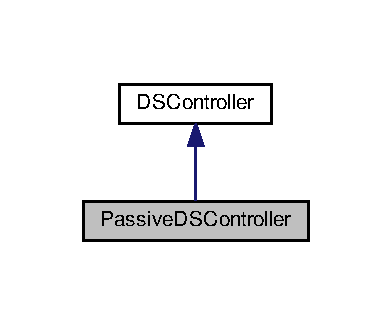
\includegraphics[width=188pt]{classPassiveDSController__inherit__graph}
\end{center}
\end{figure}


Collaboration diagram for Passive\+D\+S\+Controller\+:\nopagebreak
\begin{figure}[H]
\begin{center}
\leavevmode
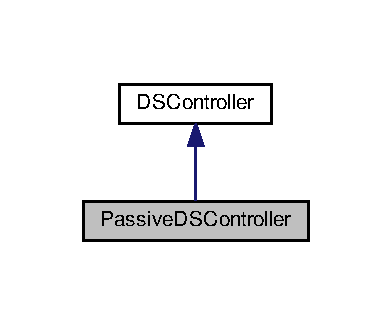
\includegraphics[width=188pt]{classPassiveDSController__coll__graph}
\end{center}
\end{figure}
\subsection*{Public Member Functions}
\begin{DoxyCompactItemize}
\item 
\hypertarget{classPassiveDSController_a8f5ced43f2163e78b5fb0c3a84711e18}{{\bfseries Passive\+D\+S\+Controller} (int dim, realtype damping\+\_\+eigval0, realtype damping\+\_\+eigval1, realtype s\+\_\+max, realtype ds, realtype dz=0.\+0)}\label{classPassiveDSController_a8f5ced43f2163e78b5fb0c3a84711e18}

\item 
\hypertarget{classPassiveDSController_a332c50c135197baf1f29f5379173343c}{void {\bfseries Update\+Passive} (const Vec \&vel, const Vec \&ref\+\_\+vel, realtype dt)}\label{classPassiveDSController_a332c50c135197baf1f29f5379173343c}

\item 
\hypertarget{classPassiveDSController_a08601ac564a6b04327db651922990515}{void {\bfseries Update\+Passive} (const Vec \&vel, const Vec \&ref\+\_\+vel\+\_\+c, const Vec \&ref\+\_\+vel\+\_\+nc, realtype dt)}\label{classPassiveDSController_a08601ac564a6b04327db651922990515}

\item 
\hypertarget{classPassiveDSController_ae764fffc8251d99def95dfbfa6013de6}{void {\bfseries reset\+\_\+storage} ()}\label{classPassiveDSController_ae764fffc8251d99def95dfbfa6013de6}

\item 
\hypertarget{classPassiveDSController_ad42b8c3c2b268d236dc4082c0bf43fdd}{realtype {\bfseries s} () const }\label{classPassiveDSController_ad42b8c3c2b268d236dc4082c0bf43fdd}

\end{DoxyCompactItemize}
\subsection*{Additional Inherited Members}


The documentation for this class was generated from the following files\+:\begin{DoxyCompactItemize}
\item 
include/passive\+\_\+ds\+\_\+controller.\+h\item 
src/passive\+\_\+ds\+\_\+controller.\+cpp\end{DoxyCompactItemize}

\hypertarget{classSmoothRise2d}{\section{Smooth\+Rise2d Class Reference}
\label{classSmoothRise2d}\index{Smooth\+Rise2d@{Smooth\+Rise2d}}
}
\subsection*{Public Member Functions}
\begin{DoxyCompactItemize}
\item 
\hypertarget{classSmoothRise2d_a50cf46c78bc33d5ed848840b824a2017}{{\bfseries Smooth\+Rise2d} (realtype xlo, realtype dx, realtype ylo, realtype dy)}\label{classSmoothRise2d_a50cf46c78bc33d5ed848840b824a2017}

\item 
\hypertarget{classSmoothRise2d_ab75a6c6e114e616487d6c05551a40a62}{realtype {\bfseries operator()} (realtype x, realtype y)}\label{classSmoothRise2d_ab75a6c6e114e616487d6c05551a40a62}

\end{DoxyCompactItemize}


The documentation for this class was generated from the following file\+:\begin{DoxyCompactItemize}
\item 
include/smooth\+\_\+truncation.\+h\end{DoxyCompactItemize}

\hypertarget{classSmoothRiseFall}{\section{Smooth\+Rise\+Fall Class Reference}
\label{classSmoothRiseFall}\index{Smooth\+Rise\+Fall@{Smooth\+Rise\+Fall}}
}
\subsection*{Public Member Functions}
\begin{DoxyCompactItemize}
\item 
\hypertarget{classSmoothRiseFall_a5ee000a0ceb6c1d273fb4db094fa376c}{{\bfseries Smooth\+Rise\+Fall} (realtype l0, realtype l1, realtype h1, realtype h0)}\label{classSmoothRiseFall_a5ee000a0ceb6c1d273fb4db094fa376c}

\item 
\hypertarget{classSmoothRiseFall_a4a2e9061daea272ad7c5de01d8205cb6}{realtype {\bfseries operator()} (realtype val)}\label{classSmoothRiseFall_a4a2e9061daea272ad7c5de01d8205cb6}

\end{DoxyCompactItemize}


The documentation for this class was generated from the following file\+:\begin{DoxyCompactItemize}
\item 
include/smooth\+\_\+truncation.\+h\end{DoxyCompactItemize}

\hypertarget{classSmoothRiseFall2d}{\section{Smooth\+Rise\+Fall2d Class Reference}
\label{classSmoothRiseFall2d}\index{Smooth\+Rise\+Fall2d@{Smooth\+Rise\+Fall2d}}
}
\subsection*{Public Member Functions}
\begin{DoxyCompactItemize}
\item 
\hypertarget{classSmoothRiseFall2d_a7ae192a8aa0ca45cd357ea98922adc52}{{\bfseries Smooth\+Rise\+Fall2d} (realtype xlo, realtype xhi, realtype dx, realtype ylo, realtype yhi, realtype dy)}\label{classSmoothRiseFall2d_a7ae192a8aa0ca45cd357ea98922adc52}

\item 
\hypertarget{classSmoothRiseFall2d_a9a02b072859fd0d0dacebde8f2d63f60}{realtype {\bfseries operator()} (realtype x, realtype y)}\label{classSmoothRiseFall2d_a9a02b072859fd0d0dacebde8f2d63f60}

\end{DoxyCompactItemize}


The documentation for this class was generated from the following file\+:\begin{DoxyCompactItemize}
\item 
include/smooth\+\_\+truncation.\+h\end{DoxyCompactItemize}

%--- End generated contents ---

% Index
\newpage
\phantomsection
\addcontentsline{toc}{chapter}{Index}
\printindex

\end{document}
